\section{TEST Data}



%------------------------------------------------
\begin{frame}[fragile]{串口打印的时间戳}
  在"report" 指令发送到主机后,有如下的代码段会被执行:
\begin{lstlisting}
/*
 report the jiffes to the  PC
*/
void report_jiffes(void)
{
  printf("master rj:\t%d\r\n", dev.local_tm.jiffies);
  printf("master rj:\t%d\r\n", dev.local_tm.jiffies);
  printf("master rj_PWM:\t%d\r\n", dev.local_tm.jiffies_pwm);
  printf("master rj_PWM:\t%d\r\n", dev.local_tm.jiffies_pwm);
 }
\end{lstlisting}

这段代码会去汇报jiffies(\textbf{本地时钟}) 和 jiffies\_pwm  {\textbf{同步时钟}}的值
给PC.
\end{frame}



%------------------------------------------------
\begin{frame}[fragile]{串口打印的时间戳}
  \begin{figure}[htbp]
  \begin{center}
  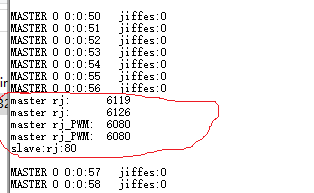
\includegraphics[width=5cm]{img/report}
  \caption{report jiffies}
  \label{report}
  \end{center}
  \vspace{-0.5em}
  \end{figure}
在输入 "report" 命令后,log 如上图(红圈里) ,结合前面的代码,可以知道:
\begin{itemize}
\item 上述代码中为了打印log , printf 的执行用时大约为 (6126-6119=7)*100us。
这里的printf 是移植的无阻塞,轻量级,全功能的printf .

\item 从机和主机有传输延时。
\end{itemize}

\end{frame}





%------------------------------------------------
\begin{frame}[fragile]{波形:未同步}

我们使
\begin{itemize}
  \item 本地时钟每8ms 使GPIOA5 电平状态 反转.这个测试通道记为CH\_LOCAL.
  \item 同步线 由主机 产生半周期为 8ms 的同步方波。 这个测试通道记为CH\_SYNC .
  \item 在从机的捕获同步线上升沿的中断处理函数中,使时钟不同步,也就是注释掉如下代码:
  \begin{lstlisting}
dev.local_tm.jiffies = dev.local_tm.jiffies_pwm;		//强等使 同步
  \end{lstlisting}

\end{itemize}


下列一些截图展示了 未同步的情况下的截图。



\end{frame}


%------------------------------------------------
\begin{frame}[fragile]{波形:未同步}

未同步的波形一\label{nosyncwave1}:

  \begin{figure}[htbp]
  \begin{center}
  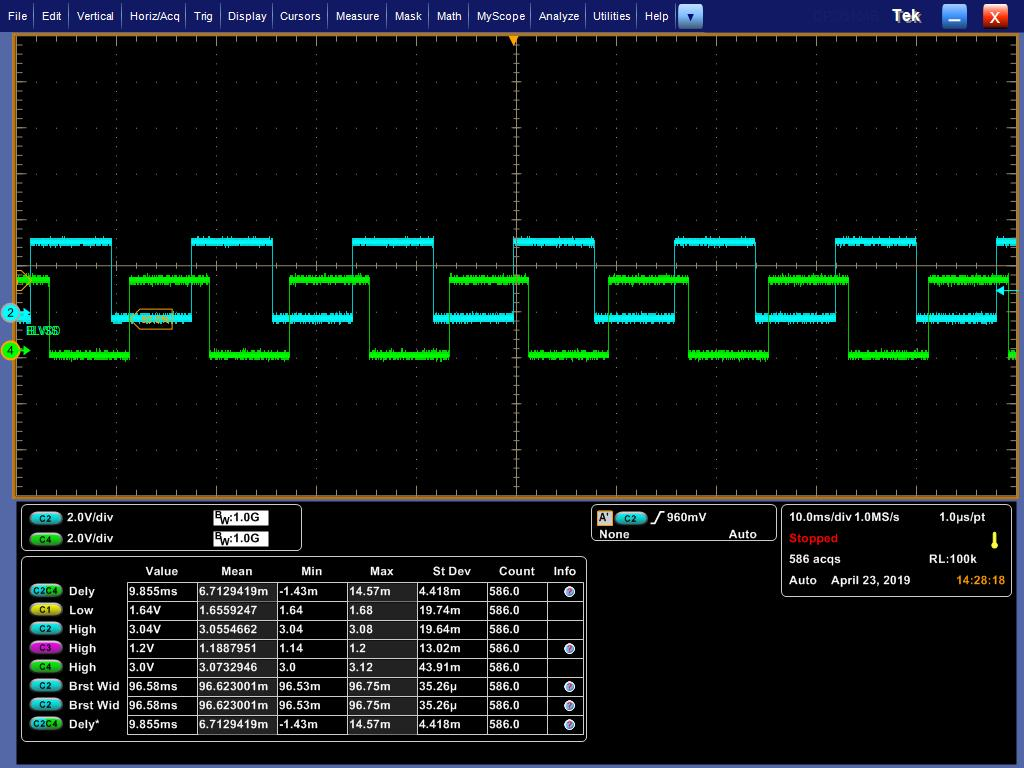
\includegraphics[width=10cm]{img/nosync1}
  \caption{report jiffies}
  \label{report}
  \end{center}
  \vspace{-0.5em}
  \end{figure}


\end{frame}



%------------------------------------------------
\begin{frame}[fragile]{波形:未同步}

未同步的波形二:

  \begin{figure}[htbp]
  \begin{center}
  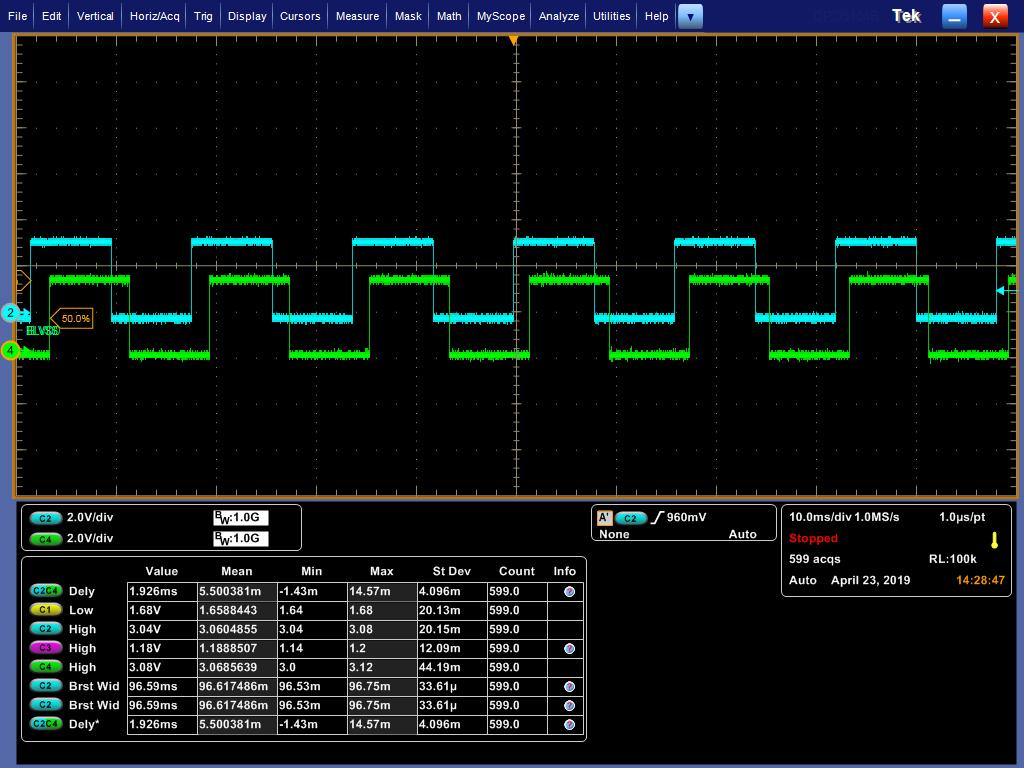
\includegraphics[width=10cm]{img/nosync2}
  \caption{report jiffies}
  \label{report}
  \end{center}
  \vspace{-0.5em}
  \end{figure}


\end{frame}


%------------------------------------------------
\begin{frame}[fragile]{波形:未同步}

未同步的波形三:

  \begin{figure}[htbp]
  \begin{center}
  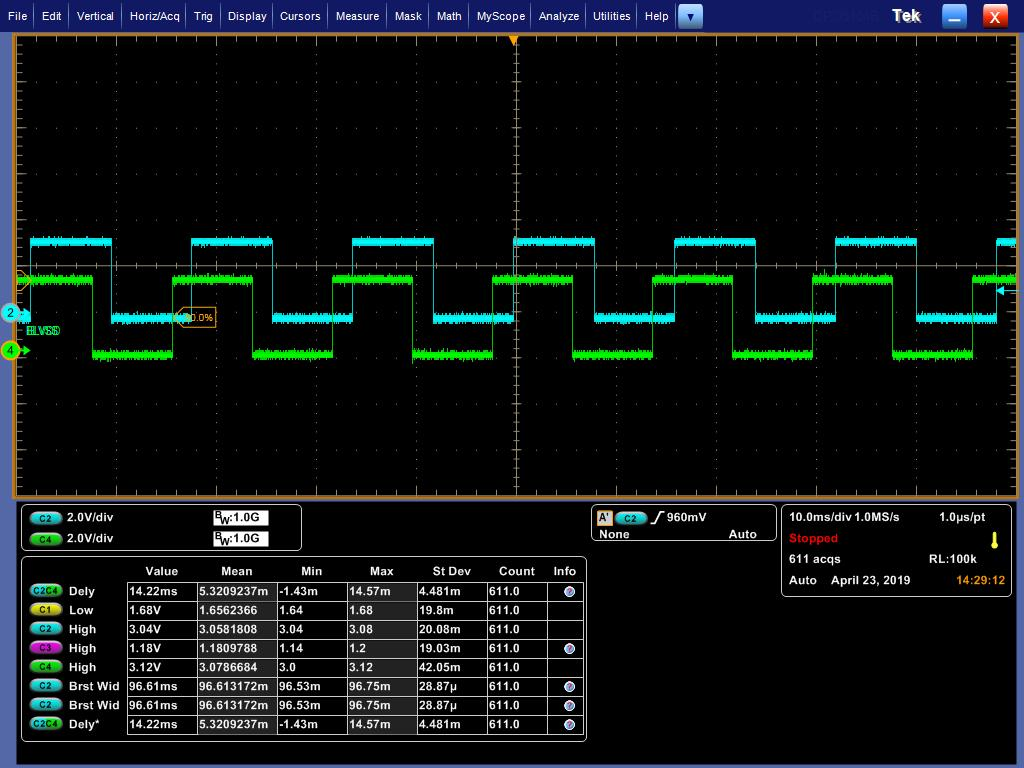
\includegraphics[width=10cm]{img/nosync3}
  \caption{report jiffies}
  \label{report}
  \end{center}
  \vspace{-0.5em}
  \end{figure}


\end{frame}


%------------------------------------------------
\begin{frame}[fragile]{波形:未同步}

未同步的波形四:

  \begin{figure}[htbp]
  \begin{center}
  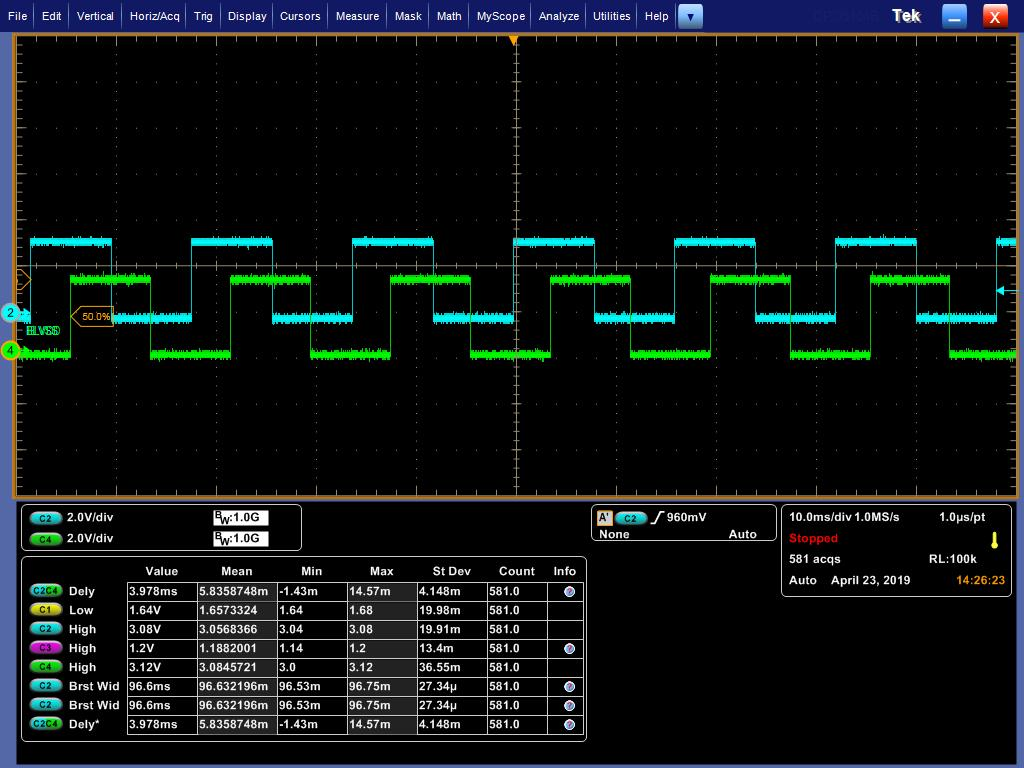
\includegraphics[width=10cm]{img/nosync4}
  \caption{report jiffies}
  \label{report}
  \end{center}
  \vspace{-0.5em}
  \end{figure}


\end{frame}


%------------------------------------------------
\begin{frame}[fragile]{未同步波形的一些说明}

把这个文档返回到未同步波形一(\ref{nosyncwave1}),然后用键盘方向键的
右键去翻页(从未同步波形一至未同步波形四)。这个时候屏幕上呈现的动画效果
比较能复原 当时示波器上的 样子。

由于 未同步 本地时钟,所以每次 误差累加,导致了这样的动态效果。

\end{frame}



%------------------------------------------------
\begin{frame}[fragile]{波形:同步}

我们使
\begin{itemize}
  \item 本地时钟每8ms 使GPIOA5 电平状态 反转.这个测试通道记为CH\_LOCAL.
  \item 同步线 由主机 产生半周期为 8ms 的同步方波。 这个测试通道记为CH\_SYNC .
  \item 在从机的捕获同步线上升沿的中断处理函数中,使时钟同步,也就是取消注释如下代码:
  \begin{lstlisting}
dev.local_tm.jiffies = dev.local_tm.jiffies_pwm;		//强等使 同步
  \end{lstlisting}

\end{itemize}


下列截图展示了 同步的情况下的截图。
\end{frame}


%------------------------------------------------
\begin{frame}[fragile]{波形:同步}

同步的波形:

  \begin{figure}[htbp]
  \begin{center}
  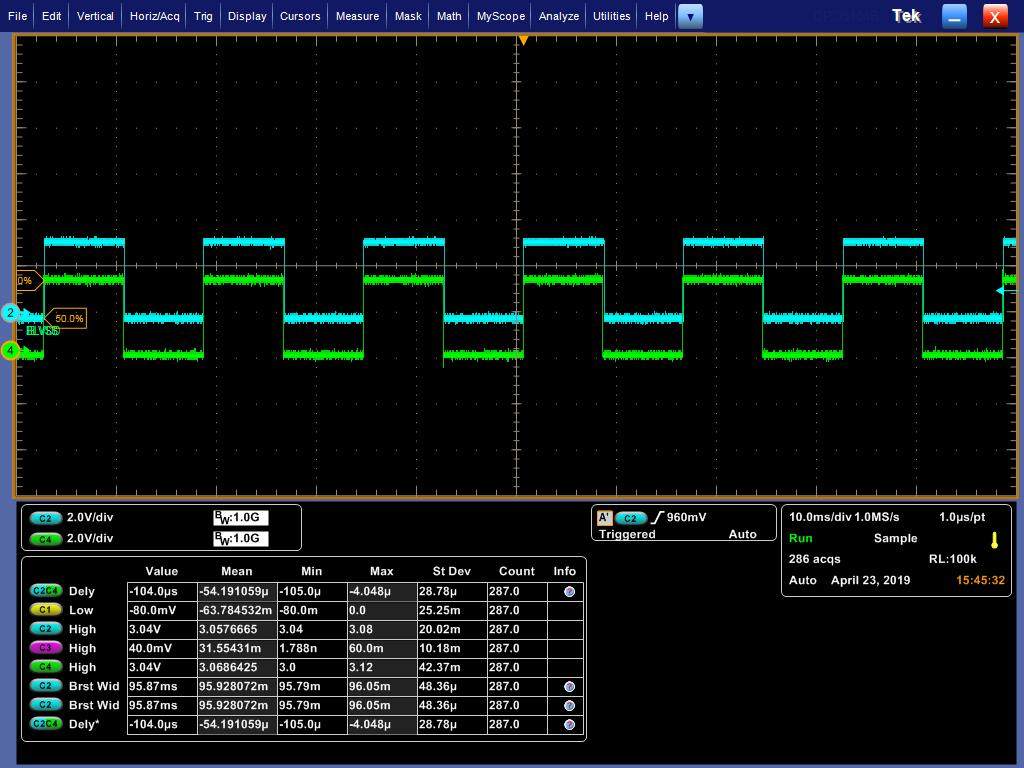
\includegraphics[width=10cm]{img/sync}
  \caption{report jiffies}
  \label{report}
  \end{center}
  \vspace{-0.5em}
  \end{figure}


\end{frame}

%------------------------------------------------
\begin{frame}[fragile]{同步波形的一些说明}

由于每次同步线上的上升沿被从机捕获后,会触发同步中断,在中断处理中,去消除每次
周期的本地时钟误差。

所以同步的波形整体看起来固定,相位 比较 一致。 但是:

如果我们放大示波器的粒度 ,会发现存在误差。下列是一些同步的误差。示波器的粒度已经为
50us 我们关注同步的前后时刻。

\end{frame}



%------------------------------------------------
\begin{frame}[fragile]{波形:同步}

同步误差:

  \begin{figure}[htbp]
  \begin{center}
  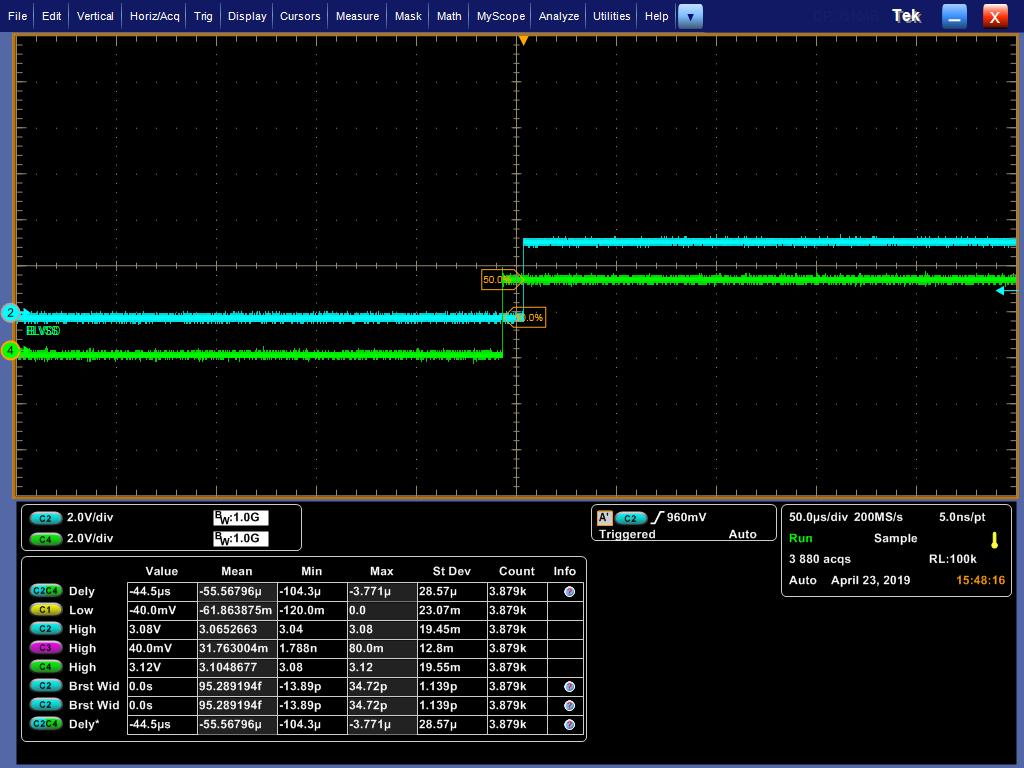
\includegraphics[width=10cm]{img/mis1}
  \caption{report jiffies}
  \label{report}
  \end{center}
  \vspace{-0.5em}
  \end{figure}


\end{frame}


%------------------------------------------------
\begin{frame}[fragile]{同步误差}

同步误差:

  \begin{figure}[htbp]
  \begin{center}
  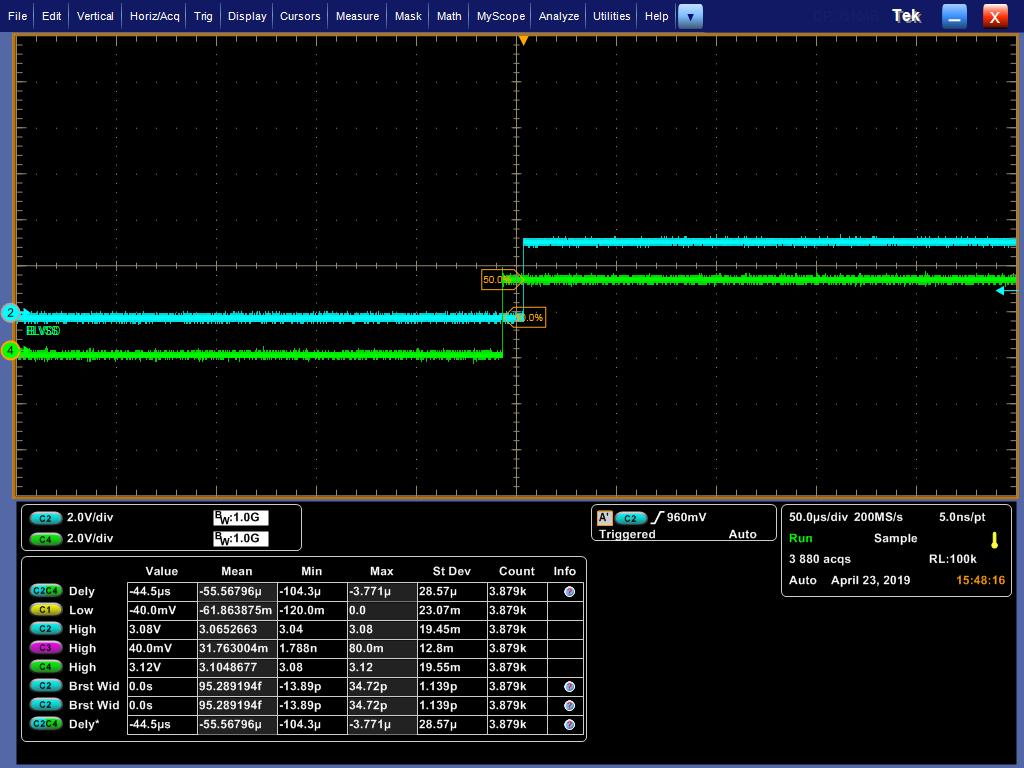
\includegraphics[width=10cm]{img/mis1}
  \caption{report jiffies}
  \label{report}
  \end{center}
  \vspace{-0.5em}
  \end{figure}


\end{frame}
%------------------------------------------------
\begin{frame}[fragile]{同步误差}

同步误差:

  \begin{figure}[htbp]
  \begin{center}
  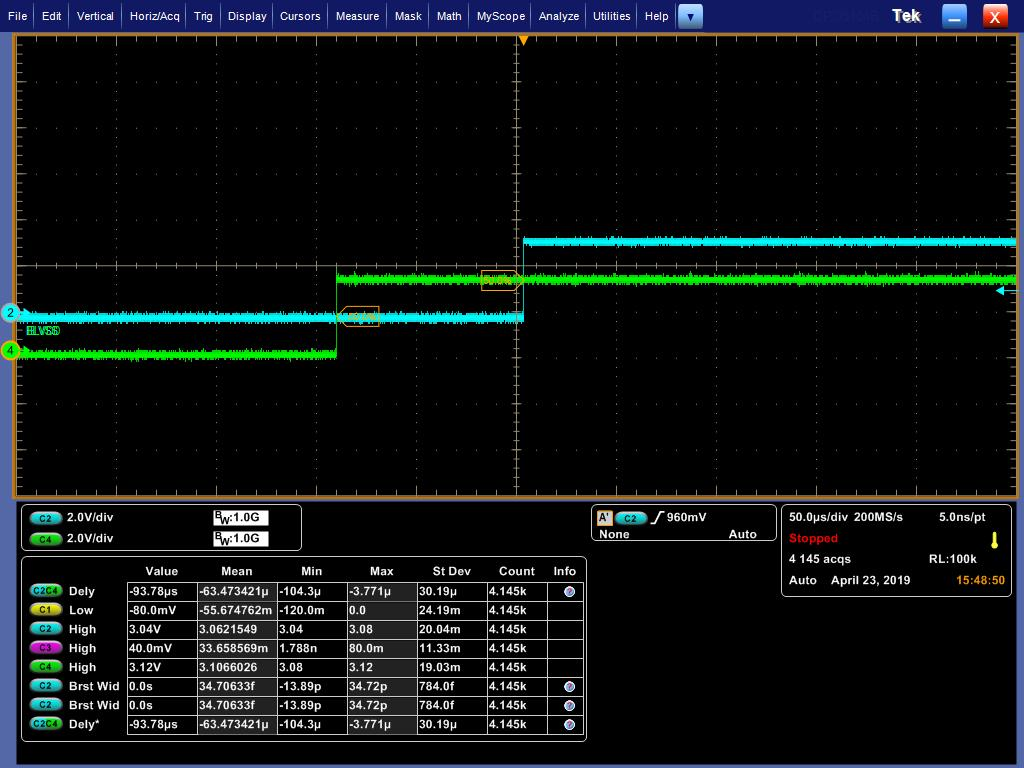
\includegraphics[width=10cm]{img/mis2}
  \caption{report jiffies}
  \label{report}
  \end{center}
  \vspace{-0.5em}
  \end{figure}


\end{frame}

%------------------------------------------------
\begin{frame}[fragile]{同步误差}

同步误差:

  \begin{figure}[htbp]
  \begin{center}
  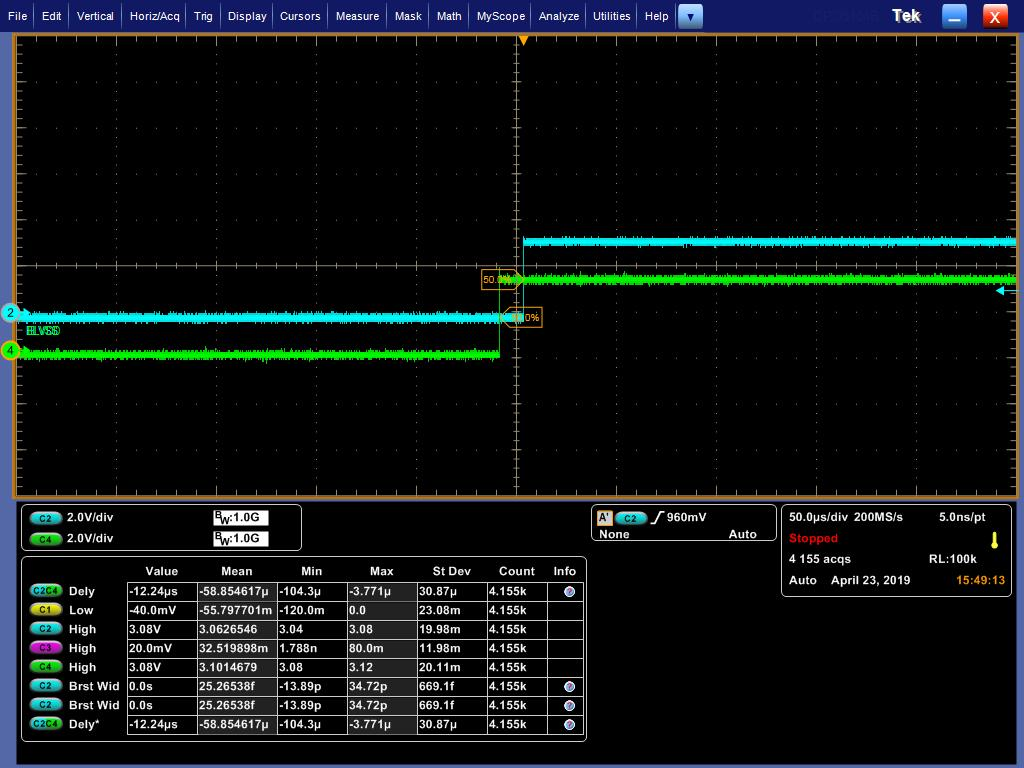
\includegraphics[width=10cm]{img/mis3}
  \caption{report jiffies}
  \label{report}
  \end{center}
  \vspace{-0.5em}
  \end{figure}

\end{frame}


%------------------------------------------------
\begin{frame}[fragile]{同步误差}

  \begin{figure}[htbp]
  \begin{center}
  
\includegraphics[width=10cm]{img/delay}
  \caption{report jiffies}
  \label{report}
  \end{center}
  \vspace{-0.5em}
  \end{figure}

上图可以看出 取样 4.155k 次,CH\_LOCAL 相比 CH\_SYNC 的相位差距最大为
-3.771 -(-104.3) = 100.529us

\end{frame}


%------------------------------------------------
\begin{frame}[fragile]{总结}

串口的数据传输会产生 一些延迟(尽管发送时无阻塞发送,在中断中接收,直接读寄存器)。 本例中我们使用的baudrate是115200*2。

纯软件的CRC 校验 必然带来一定的延时,如果需要校验,在本项目中需要实现CRC硬件外设的驱动。

demo同步后的误差 经过多次测试 ,其中有变换主从角色,最大的误差在500us 以内。最常见的是
300us 以内.

本次测试 代码逻辑不复杂,实时性的处理都在中断上下文,而STM32F4 使用Cortex M4的Nested Vectored Interrupt Controller (NVIC) 实时性非常高 ,应该少有优化空间。

\end{frame}
